\documentclass{article}

\usepackage{geometry}
\usepackage{amsmath}
\usepackage{graphicx}
\usepackage{listings}
\usepackage{hyperref}
\usepackage{multicol}
\usepackage{fancyhdr}
\pagestyle{fancy}
\hypersetup{ colorlinks=true, linkcolor=black, filecolor=magenta, urlcolor=cyan}
\geometry{ a4paper, total={170mm,257mm}, top=20mm, right=20mm, bottom=20mm, left=20mm}
\setlength{\parindent}{0pt}
\setlength{\parskip}{1em}
\renewcommand{\headrulewidth}{0pt}
\lhead{Competitive Programming - ITB}
\fancyfoot[CE,CO]{\thepage}
\lstset{
    basicstyle=\ttfamily\small,
    columns=fixed,
    extendedchars=true,
    breaklines=true,
    tabsize=2,
    prebreak=\raisebox{0ex}[0ex][0ex]{\ensuremath{\hookleftarrow}},
    frame=none,
    showtabs=false,
    showspaces=false,
    showstringspaces=false,
    prebreak={},
    keywordstyle=\color[rgb]{0.627,0.126,0.941},
    commentstyle=\color[rgb]{0.133,0.545,0.133},
    stringstyle=\color[rgb]{01,0,0},
    captionpos=t,
    escapeinside={(\%}{\%)}
}

\begin{document}

\begin{center}
    \section*{Penyebaran Corona (Version 2)} % ganti judul soal

    \begin{tabular}{ | c c | }
        \hline
        Batas Waktu  & 2s \\    % jangan lupa ganti time limit
        Batas Memori & 512MB \\  % jangan lupa ganti memory limit
        \hline
    \end{tabular}
\end{center}

\subsection*{Deskripsi}

Di suatu perumahan, virus berbahaya \textit{corona} telah masuk ke salah satu rumah. Diketahui bahwa di perumahan tersebut terdapat $N$ rumah yang setiap rumah dinomori dari $1$ sampai $N$ dan terdapat tepat $N - 1$ jalan antara rumah, sehingga bisa dibilang perumahan ini seperti sebuah \textit{tree} pada suatu graf. Namun, sayang sekali Anda tidak tahu pada rumah mana virus \textit{corona} terkena, sehingga Anda penasaran seandainya virus tersebut ada pada rumah nomor-$i$ maka jaraknya ke rumah lain bernomor-$j$ adalah berapa ?

\subsection*{Format Masukan}

Baris pertama terdiri dari satu bilangan bulat positif $N, Q$ ($2 \leq N, Q \leq 100000$), menyatakan banyaknya rumah yang ada dan banyaknya pertanyaan yang Anda miliki.

$N-1$ baris berikutnya terdiri dari 2 bilangan $u, v$ ($1 \leq u, v \leq n$ dan $u \neq v$) yang artinya ada jalan dari rumah nomor $u$ ke rumah nomor $v$

$Q$ baris berikutnya terdiri dari 2 bilangan $u, v$ ($1 \leq u, v \leq n$ dan $u \neq v$) yang artinya jika seandainya ada virus di kota-$u$ maka berapakah jaraknya ke kota-$v$

\subsection*{Format Keluaran}

Keluarkan $Q$ baris, dengan setiap baris-$i$ menjawab pertanyaan ke-$i$

\begin{multicols}{2}
\subsection*{Contoh Masukan}
\begin{lstlisting}
7 5
1 7
1 2
1 3
3 5
3 4
5 6
1 4
2 3
3 7
5 6
7 4

\end{lstlisting}
\columnbreak
\subsection*{Contoh Keluaran}
\begin{lstlisting}
2
2
2
1
3
\end{lstlisting}
\vfill
\null
\end{multicols}
\pagebreak
\subsection*{Penjelasan}
Ilustrasi perumahan adalah sebagai berikut:
\begin{center}
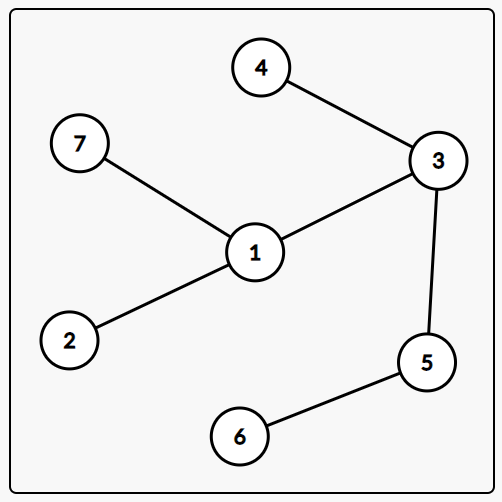
\includegraphics[scale=0.6]{graf}
\end{center}
Kita akan dapat bahwa:
\begin{itemize}
	\item Jarak rumah-$1$ ke rumah-$4$ adalah $2$
	\item Jarak rumah-$2$ ke rumah-$3$ adalah $2$
	\item Jarak rumah-$3$ ke rumah-$7$ adalah $2$
	\item Jarak rumah-$5$ ke rumah-$6$ adalah $1$
	\item Jarak rumah-$7$ ke rumah-$4$ adalah $3$
\end{itemize}


\pagebreak

\end{document}